\subsection{ENVELOPING ALGEBRA OF A LIE SUBALGEBRA}

Let g be a Lie algebra over K, h a subalgebra of g and \(\sigma\) , \(\sigma'\) the canonical mappings of g, h into their enveloping algebras U, V. Then the canonical injection i of h into g defines a homomorphism i, called canonical, of V into U such that \(\sigma \circ i = i \circ \sigma'\) . The algebra \(i(\mathrm{V})\) is generated by 1 and \(\sigma(\mathfrak{h})\) . We shall see (no. 7, Corollary to Theorem 5) that i is injective in important cases.

If \(\mathfrak{h}\) is an ideal of \(\mathfrak{g}\) , the left ideal of U generated by \(\sigma(\mathfrak{h})\) coincides with the right ideal generated by \(\sigma(\mathfrak{h})\) , in other words it is a two-sided ideal R. This follows since, for \(x \in \mathfrak{h}\) and \(x' \in \mathfrak{g}\) ,

\[
\sigma (x) \sigma (x ^ {\prime}) = \sigma (x ^ {\prime}) \sigma (x) + \sigma ([ x, x ^ {\prime} ])
\]

and \([x, x'] \in \mathfrak{h}\) .

PROPOSITION 3. Let \(\mathfrak{h}\) be an ideal of \(\mathfrak{g}, p\) the canonical homomorphism of \(\mathfrak{g}\) onto \(\mathfrak{g} / \mathfrak{h}\) and W the enveloping algebra of \(\mathfrak{g} / \mathfrak{h}\) . The homomorphism:

\[
\tilde {p}: \mathrm{U} \rightarrow \mathrm{W}
\]

defined canonically by \(p\) is surjective and its kernel is the ideal \(R\) of \(U\) generated by \(\sigma(h)\) .

Let \(\sigma''\) be the canonical mapping of \(g/h\) into W. The commutative diagram:

\pandocbounded{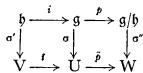
\includegraphics[keepaspectratio]{images/part001_4ab4ddcc.jpg}}

proves that \(\tilde{p}\) is zero on \(\sigma(\mathfrak{h})\) and hence on R. Let \(\psi\) be the canonical homomorphism of U onto U/R. There exists a homomorphism \(\phi\) of U/R

\pandocbounded{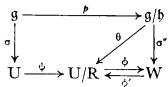
\includegraphics[keepaspectratio]{images/part001_c6a5c19d.jpg}}

into W such that \(\tilde{p} = \phi \circ \psi\) . The mapping \(\psi \circ \sigma\) of \(g\) into U/R is an \(\alpha\) -mapping and is zero on \(h\) and hence defines an \(\alpha\) -mapping \(\theta\) of \(g / h\) into U/R such that \(\theta \circ p = \psi \circ \sigma\) . Then \(\phi \circ \theta \circ p = \phi \circ \psi \circ \sigma = \sigma'' \circ p\) . Hence \(\phi \circ \theta = \sigma''\) . There exists (no. 1, Proposition 1) one and only one homomorphism \(\phi'\) of W into U/R mapping 1 to 1 and such that \(\theta = \phi' \circ \sigma''\) . Then \(\phi' \circ \phi \circ \theta = \phi' \circ \sigma'' = \theta\) and \(\phi \circ \phi' \circ \sigma'' = \phi \circ \theta = \sigma''\) and hence \(\phi' \circ \phi\) and \(\phi \circ \phi'\) are the identity mappings of U/R and W respectively. This completes the proof.

U/R is identified with W under the isomorphism \(\phi\) . Then the canonical mapping \(\sigma''\) of \(g/h\) into W is identified with \(\theta\) , that is with the mapping of \(g/h\) into U/R derived from \(\sigma\) by taking quotients.

